

% Slides for 2024-02-07
% To create a slide with a graphic:
% 1. Add the graphic to this folder (named picture.png)
% 2. Use the following:
\begin{frame}{Quick Updates}
    \begin{itemize}
        \item template matching data human verified
        \item IR response augmentation tested, train on Weekend
        \item Collecting XC data for SDSC
    \end{itemize} 
\end{frame}

\begin{frame}{How much Labeling Needed to Identify All True Positives? pt 1}
    \centering
    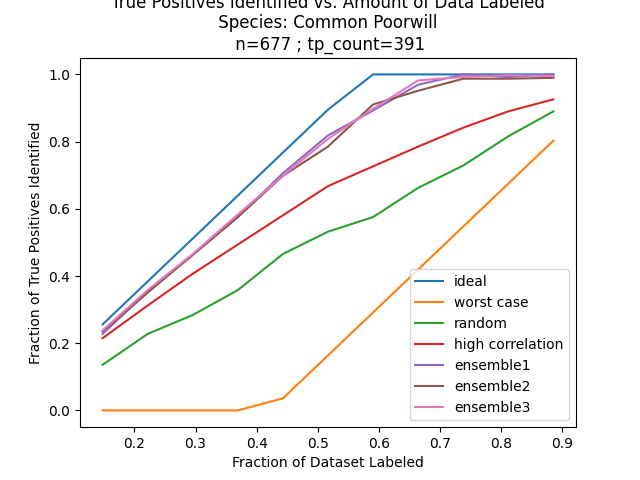
\includegraphics[height=0.7\textheight,width=0.7\textwidth,keepaspectratio]{images/aid/poorwill.png}
\end{frame}

\begin{frame}{How much Labeling Needed to Identify All True Positives? pt 2}
    \centering
    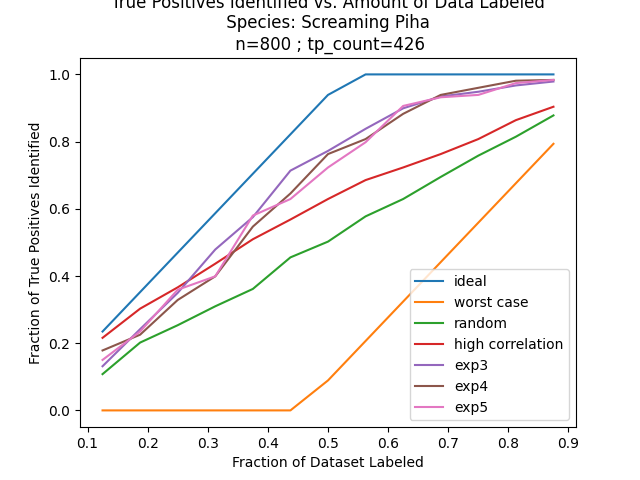
\includegraphics[height=0.7\textheight,width=0.7\textwidth,keepaspectratio]{images/aid/piha.png}
\end{frame}

\begin{frame}{How much Labeling Needed to Identify All True Positives? pt 3}
    \centering
    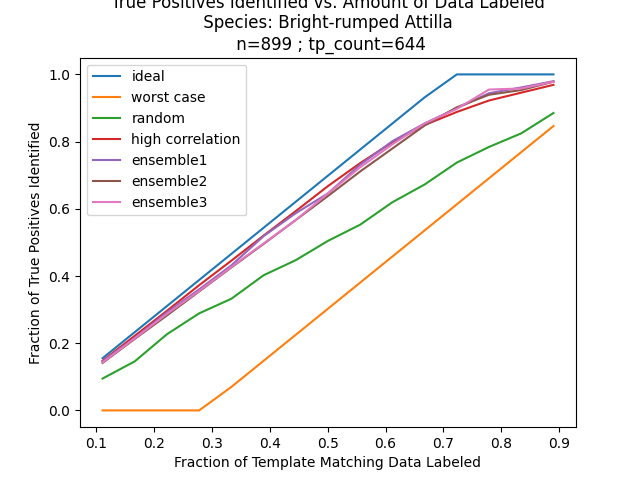
\includegraphics[height=0.7\textheight,width=0.7\textwidth,keepaspectratio]{images/aid/attilla.png}
\end{frame}

\begin{frame}{How Can We Pick Best Data to Label? pt 1}
    \centering
    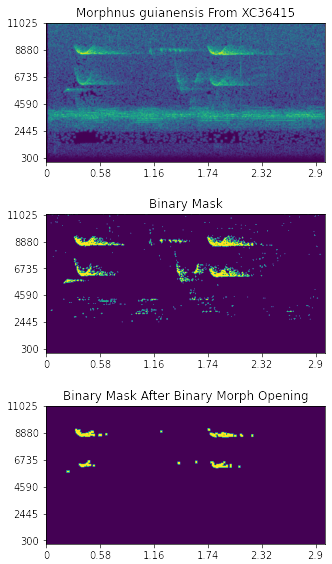
\includegraphics[height=1\textheight,width=1\textwidth,keepaspectratio]{images/aid/paper.png}
\end{frame}

\begin{frame}{How Can We Pick Best Data to Label? pt 2}
    \centering
    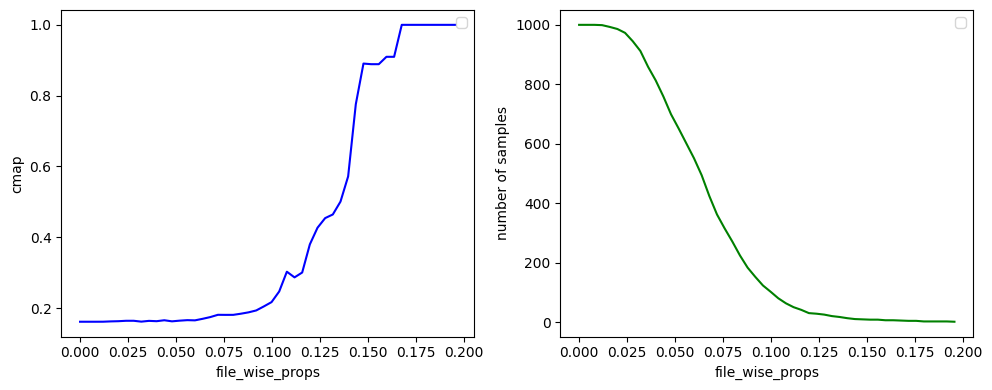
\includegraphics[height=0.9\textheight,width=1\textwidth,keepaspectratio]{images/aid/image (4).png}
\end{frame}

\begin{frame}{Dylan Thesis}
    \centering
    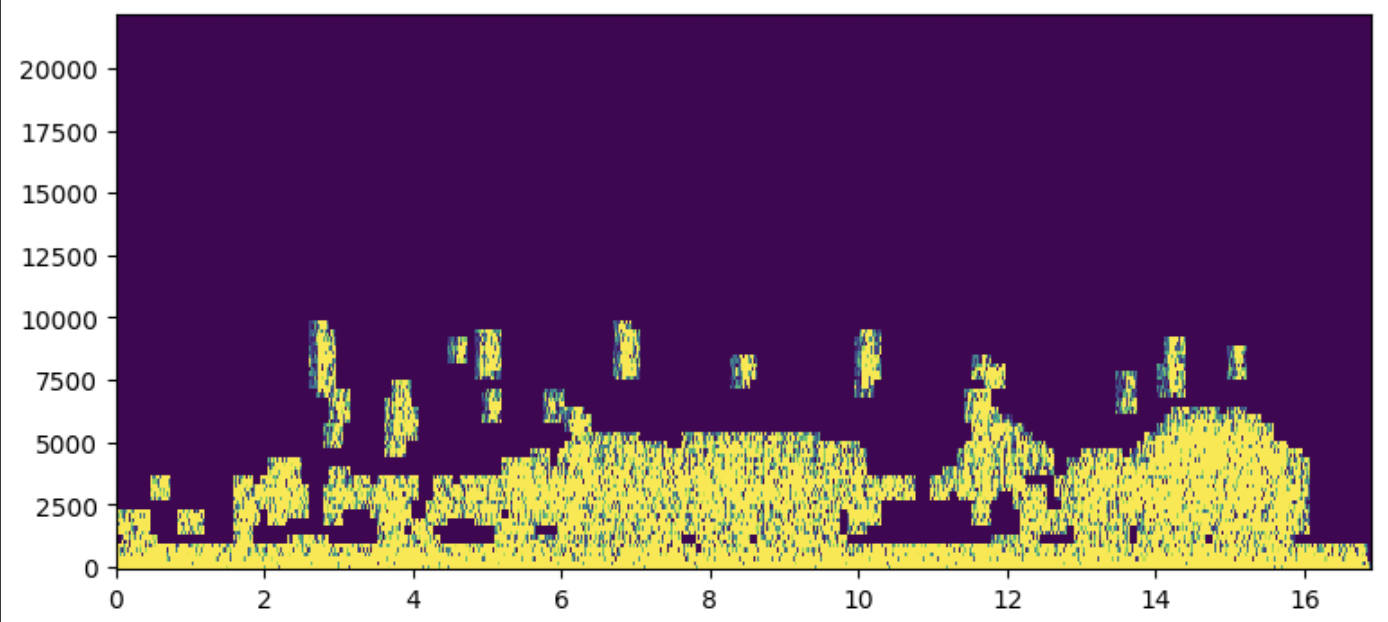
\includegraphics[height=0.7\textheight,width=0.7\textwidth,keepaspectratio]{images/aid/dylan-aid-2-7.png}
\end{frame}


% To create a slide, use the following:
% \begin{frame}{TITLE}
%     BODY
% \end{frame}

% To create a slide with a bullet list, use the following:
% \begin{frame}{TITLE}
%     \begin{itemize}
%         \item ITEM 1
%         \item ITEM 2
%     \end{itemize}    
% \end{frame}

% To create a slide with numbered list, use the following:
% \begin{frame}{TITLE}
%     \begin{enumerate}
%         \item ITEM 1
%         \item ITEM 2
%     \end{enumerate}
% \end{frame}

% To create a slide with a graphic:
% 1. Add the graphic to this folder (named picture.png)
% 2. Use the following:
% \begin{frame}{TITLE}
%     \centering
%     \includegraphics[height=0.7\textheight,width=0.7\textwidth,keepaspectratio]{picture.png}
% \end{frame}

% To create a slide with two columns, use the following:
% \begin{frame}{TITLE}
%     \begin{columns}
%         \begin{column}{0.5\textwidth}
%             COLUMN 1 BODY
%         \end{column}
%         \begin{column}{0.5\textwidth}
%             COLUMN 2 BODY
%         \end{column}
%     \end{columns}
% \end{frame}
